\documentclass[a4paper,10pt]{article}
\usepackage[utf8]{inputenc}
\usepackage[english]{babel}
\usepackage[onehalfspacing]{setspace}
\usepackage{float}
\usepackage{amsmath}

\usepackage[nottoc]{tocbibind} %Adds "References" to the table of contents
\usepackage[titletoc]{appendix}

\usepackage{graphicx}
\usepackage{hyperref}
\usepackage{multirow}

%\graphicspath{/home/trung/Pictures/} \usepackage{float}
\hypersetup{
    colorlinks=true,
    linkcolor=blue,
    filecolor=magenta,      
    urlcolor=cyan,
}
%Document title, author and date (empty)
\title{HT Heat Pump WP2 report}
\author{Trung Nguyen}
\date{}

%Beginning of the document
\begin{document}

\maketitle

\tableofcontents

\section{Introduction}
WP2 report: support the HP design by making a Simulation system.\\
Activities relates to this work packages:
- Preparation of the conceptual design.\\
- System modelling: develop a dynamic model of HT Heat pump. Creating a load profile of office building, D.M.H, ...etc.
- 
 -Draft refrigeration cycle report 

o Model of the refrigeration cycle 

o Simulation of reference cases 

o Associated operating conditions compressor. 

• Package of requirements and compressor test plan 

• Overview of components with substantiation.


%-------------------------------------------

\section{Refrigeration cycle}


%-----------------------------------------------------------------------
\section{ Model of the refrigeration cycle}



%________________________________________________________
\section{Office building load profile}

For nearly energy-neutral buildings (bijna energieneutrale kantoorgebouwen 'BENG') specific requirements for energy consumption will apply from 2021.The maximum energy requirement for heating, cooling and lighting for utility buildings, is 50 kWh/$m^2$ per year. The number is increased to 65 kWh/$m^2$ per year for healthcare buildings.This excludes the energy consumption for office equipment \href{https://www.energievastgoed.nl/benchmarktool/}{[1]}.\\
The average gas consumption for office building is around 17 $m^3$/$m^2$ (figure 1) for the building with the construction year between 1977 and 1989.The report from ECN has calculated the buildings with an office function cover a total of 87 million m2. This concerns 68,000 buildings in the Netherlands. Gas consumption amounts to 955 million m3 (30 PJ) and electricity to 7800 million kWh (28 PJ). These values are the most accurate available at the moment.  
\href{https://www.energievastgoed.nl/2017/02/14/benchmark-energieverbruik-gebouwen/}{[2],[3]}.

\begin{figure}[ht]
\centering
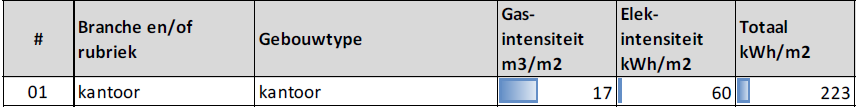
\includegraphics[width=1\columnwidth]{pictures/ECN.png}
\caption[Short title]{Energy Consumption}
\label{fig:ff1}\end{figure}

% \begin{figure}[ht]
% \centering
% 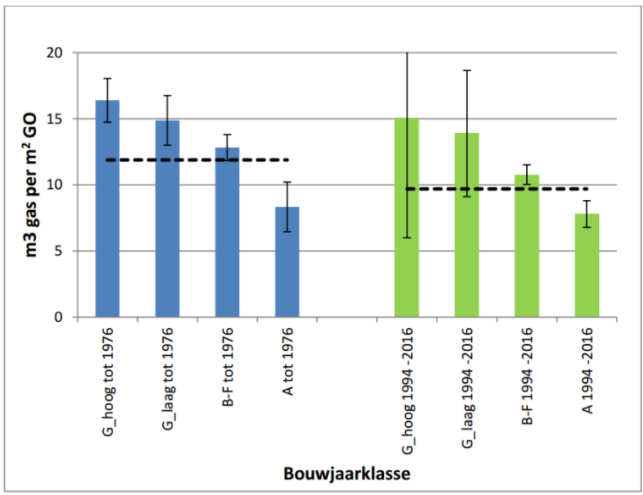
\includegraphics[width=1\columnwidth]{pictures/gas use.png}
% \caption[Short title]{Office building gas consumption per m2 }
% \label{fig:ff1}\end{figure}

The references building has been selected:

    \begin{itemize}
      \item Construction year: 1977-1989.
      \item Surface $m^2$: 500
      \item Gas consumption: 17 $m^3$/$m^2$
      \item T{\_outside} : out door temperature from NEN5060\texttt{\_}2018 with 1 hour sampling rate for 1 year long.
    \end{itemize}
Assume that there is no heating needed, when out side temperature is 15 degree. The heating line is set on 14 $^o$C.
The office is 500 $m^2$ the gas consumption is around 8500  $m^3$ gas or 82450 kwh (1 $m^3$ equals approximately 9.7 kWh).\\
The (“graaduren”) $^o$C per hour necessary to achieve the right inside temperature.


%\[Q_{per{\_}degree} = \frac{97000}{\sum{(14 - T_{outside})}}\] 

\begin{equation}
Q_{per{\_}degree}=\frac{97000}{\sum(14 - T_{outside})}
\end{equation}

Energy demand profile is calculated with period of 1 hour for the whole year.

\begin{equation}
Q_{profile}=Q_{per{\_}degree}*{(14 - T_{outside})}
\end{equation}

The energy demand profile is showed in figure 1.

\begin{figure}[H]
\centering
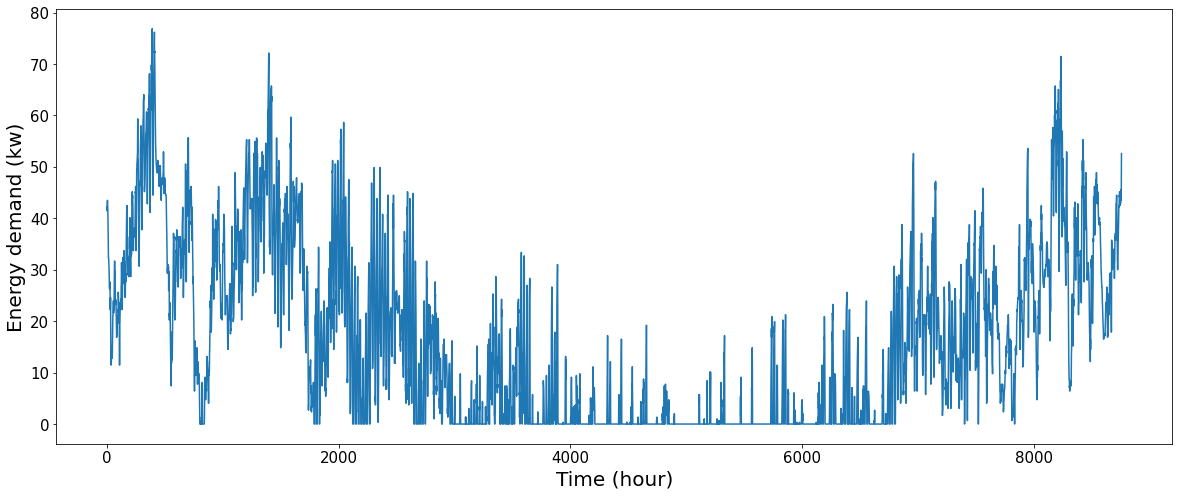
\includegraphics[width=1\columnwidth]{pictures/Q_profile.png}
\caption[Short title]{Energy Consumption of office building.}
\label{fig:ff2}\end{figure}

%__________________________________________________

\section{Apartment Building load profile}
\subsection{Heating profile}

The apartment building (Flatwoningen (overig) Gebouwd) build in the period 1965-1974 which represent 1.8 \texttt{\%} of the dutch housing stock [5] (highest number in the flatwoningen category) will be selected. Houses in this category often have 2 to 4 rooms.The average gas consumption for this type of apartment (energy label C) is 829 $m^3$/year with the average usage area is 77 m2 and 2.8 people in the house. Label C has been selected because the focus of heat pump heating will be on the renovated house with good insulation. The property features are showing in figure 3.

\begin{figure}[H]
\centering
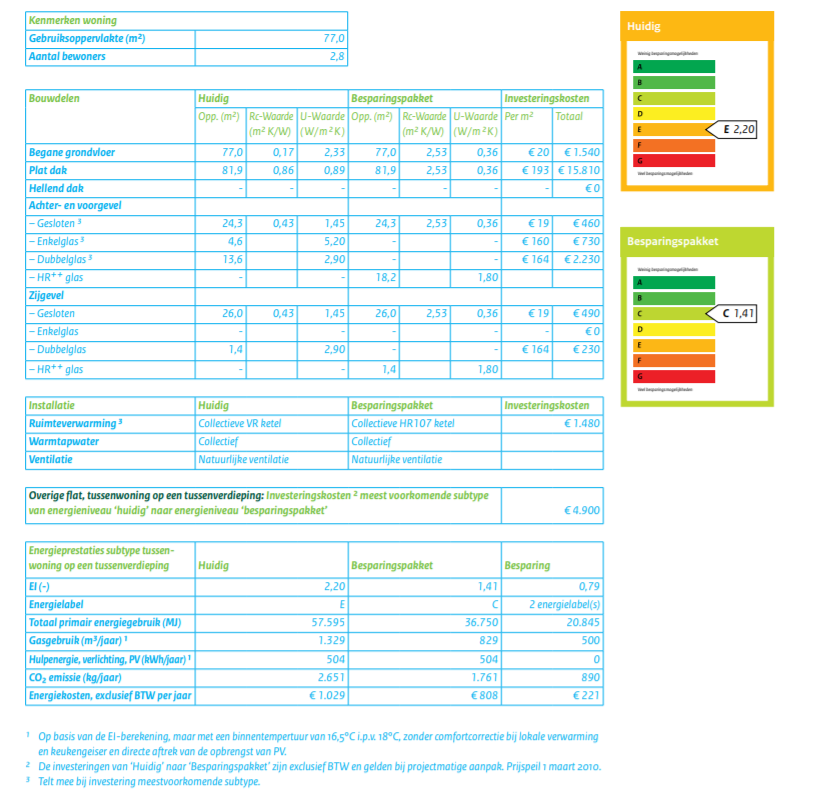
\includegraphics[width=1\columnwidth]{pictures/property features.png}
\caption[Short title]{property features [5].}
\label{fig:ff3}\end{figure}
From statista.com (figure 4)one person use approximately 120 liters of water per day therein one third of the water is used for showering and bathing. The rest for washing, toilet and cooking.

\begin{figure}[H]
\centering
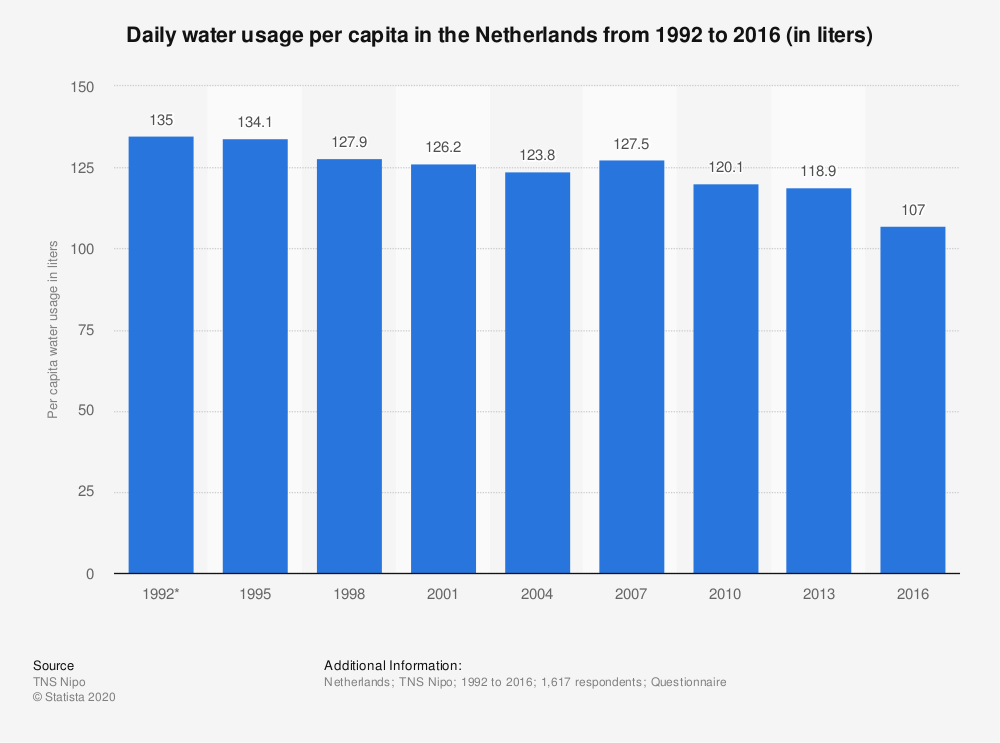
\includegraphics[width=1\columnwidth]{pictures/daily water usage.png}
\caption[Short title]{daily water usage by capital.}
\label{fig:ff4}\end{figure}


If one person use around 60 liters of hot tap water at 40 degree per day. The energy use by one person can be calculated:

\begin{equation}
Q = m.c.\Delta T
\end{equation}
\\
60 liters $\approx$ 60 kg of water.\\
c = 4.19 kj/kg.K specific heat capacity of water.\\
$\Delta$T: temperature different: 40 - 10 = 30 $^o$C.\\ 
\\
At the results one person will consume 2.095kwh per day for hot tap water. 2.8 people will consume 5.866 kwh per day.\\
Cross check with "VERORDENING (EU) Nr. 814/2013 VAN DE COMMISSIE van 2 augustus 2013". The hot water capacity M profile (will be discussed in next chapter) has a sum of energy use for tap water per day 5,845 kwh.

\begin{figure}[H]
\centering
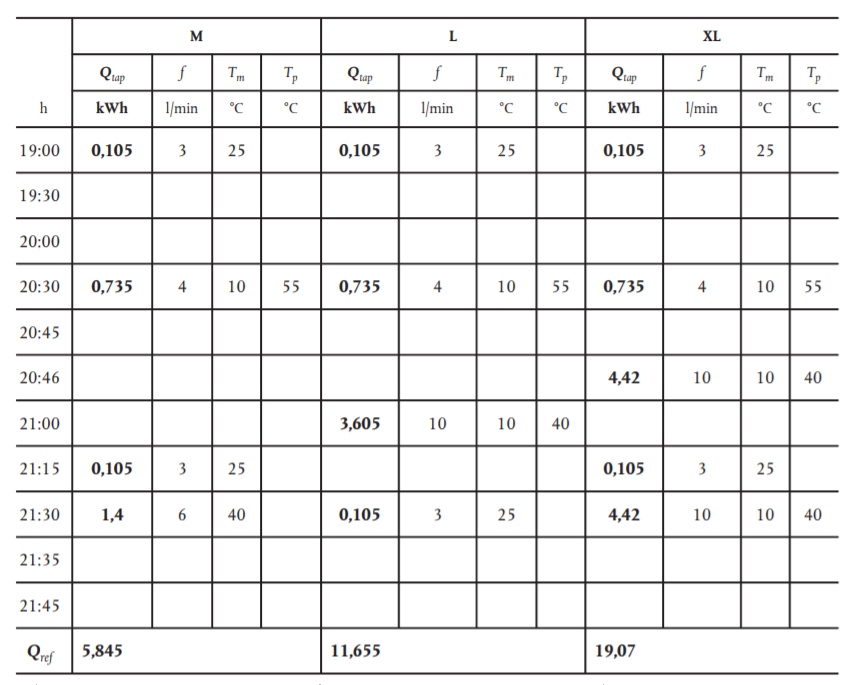
\includegraphics[width=1\columnwidth]{pictures/hot tap water.png}
\caption[Short title]{example hot tap water profile.}
\label{fig:ff5}\end{figure}


% \begin{figure}[H]
% \centering
% 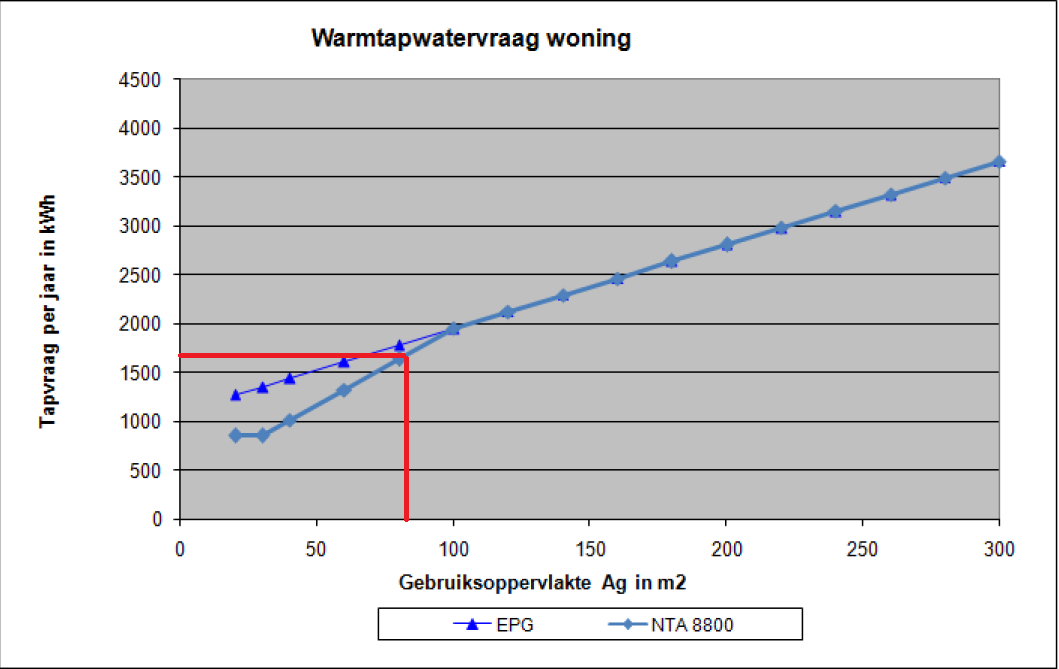
\includegraphics[width=1\columnwidth]{pictures/Tap_water_perm2.png}
% \caption[Short title]{Energy Consumption of the Apartment}
% \label{fig:ff6}\end{figure}.


An average energy use for heating is 5907.875 kwh per apartment. The heat demand profile for apartment building will be calculated follow equation (2) and (3). 

\begin{figure}[H]
\centering
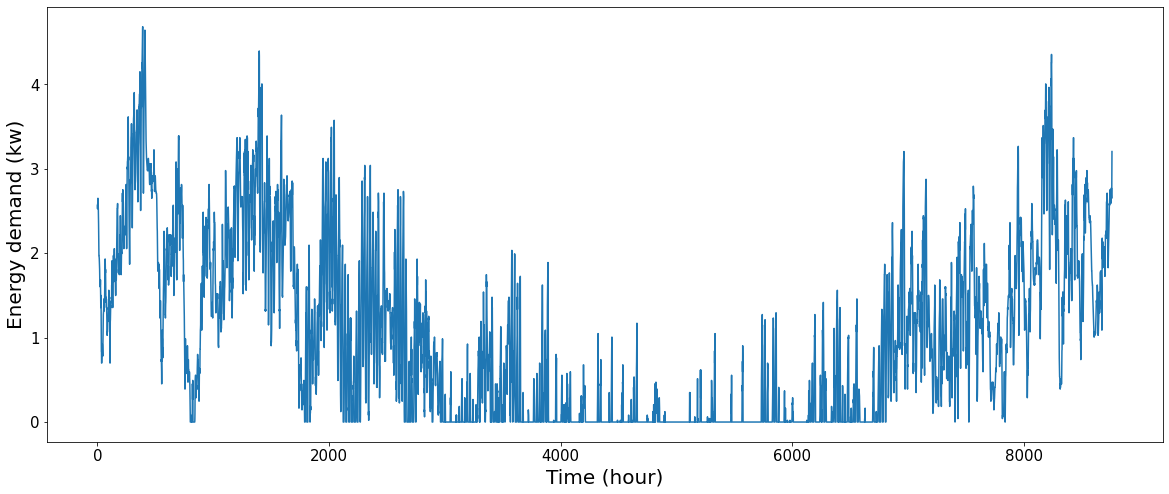
\includegraphics[width=1\columnwidth]{pictures/Apartment_profile.png}
\caption[Short title]{Energy Consumption of the Apartment.}
\label{fig:ff6}\end{figure}




%________________________________________________________
\subsection{Hot tap water profile}
 
 
A normal dutch house using CW label 3 or 4 (Appendix A). Therefore capacity profile M will be selected as a reference.\\
Capacity profile definition:
Annex III of the EU regulation[3] describes a capacity profile for a 24-hour measurement cycle intended for checking compliance with the requirements.\\
This capacity profile is as follows:

\begin{itemize}
      \item No hot water consumption from 9:35 PM to 7 AM.
      \item From 07:00 to 21:30 hot water consumption according to a precisely defined tap profile.
    \end{itemize}
An example calculation is shown below: 

\begin{figure}[H]
\centering
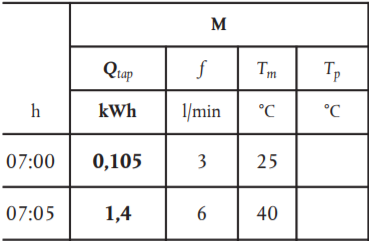
\includegraphics[width=0.6\columnwidth]{pictures/Tap_water example.png}
\caption[Short title]{Tap water example [4].}
\label{fig:ff7}\end{figure}
At 7.00 $Q_{tap}$ is 0.105 kwh with the flow rate at 3 liters  per minutes and temperature added is 25 degree.

\[m = \frac{3600.Q}{c.\Delta T}\]

m = 6 liters(kg), c=4.19 kj/kg.K. Therefore 2 minutes of tap water has been used at 7.00 AM

The hot tap water profile M for 1 day is showing in figure 10:

\begin{figure}[H]
\centering
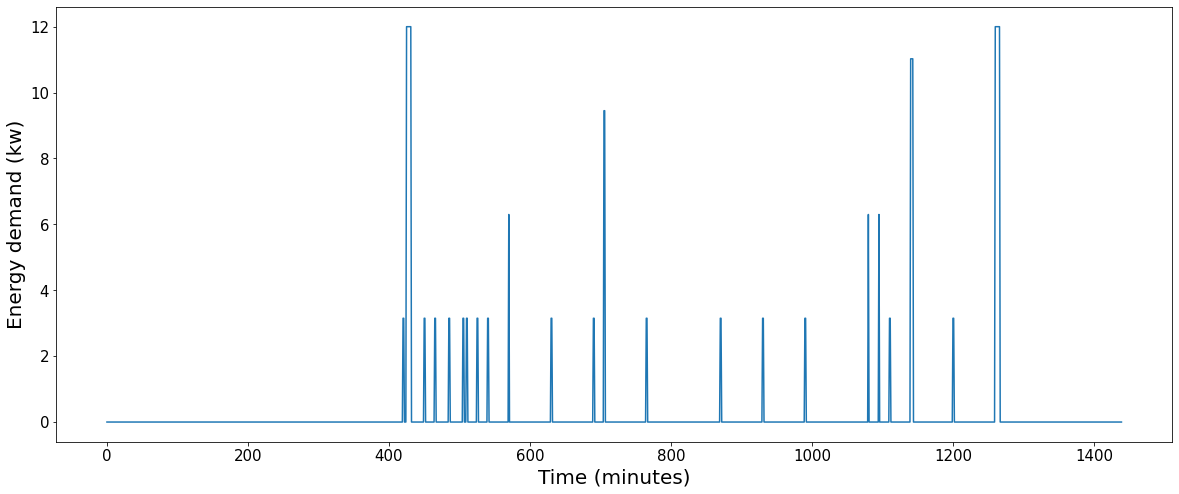
\includegraphics[width=1\columnwidth]{pictures/hot_tap_water_profile_M.png}
\caption[Short title]{hot tap water profile M.}
\label{fig:ff8}\end{figure}

\subsection{Simulation profile for the entire building}

The simulation is base on the assumption of the apartment building with 24 residential apartments.
The hot tap water demand for 24 apartments will be calculated base on the calculation rules public in kennisbank isso 55.

\begin{figure}[H]
\centering
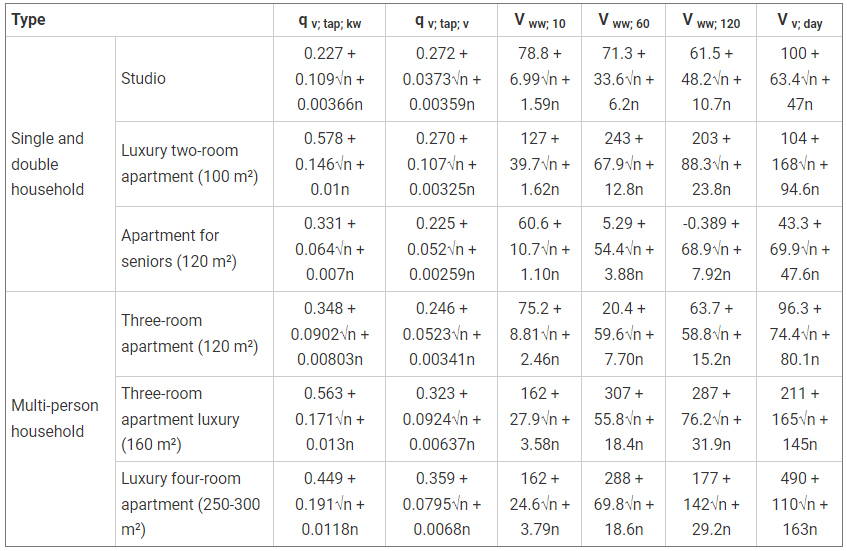
\includegraphics[width=1\columnwidth]{pictures/Calculation rules for hot tap water demand for apartment buildings.png}
\caption[Short title]{Calculation rules for hot tap water demand for apartment buildings[6].}
\label{fig:ff9}\end{figure}
The instantaneous hot water requirement for an hour is:

\begin{figure}[H]
\centering
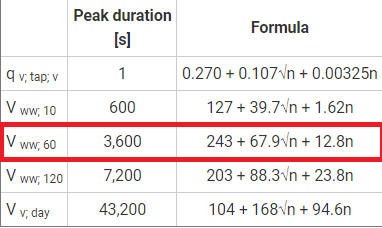
\includegraphics[width=0.5\columnwidth]{pictures/tap water demand in an hour.png}
\caption[Short title]{Calculation rules for hot tap water demand for an hour[6].}
\label{fig:ff10}\end{figure}

\begin{equation}
V_{WW;60} = 243 + 67.9\sqrt{n} + 12.8n
\end{equation}

$V_{WW;60}$: volume flow of hot water in 60 minutes
n: number of apartments

The hot tap water profile for building apartment are shown below:

%---------------------------------------------------------------------
%Example of the multicolumn command
\begin{table}[h!]
\centering
\begin{tabular}{|p{3cm}|p{3cm}|}
\hline
\multicolumn{2}{|c|}{1 day hot tap water usage} \\
\hline
Time& $Q_{tap}$ (kwh)\\ % & Use periods(hour)
 \hline
 07:00	& 38.64   \\ % &1.1
 08:00  & 10.08   \\ % &0.8
 09:00	& 5.04    \\ % &0.4
 10:00  & 2.52    \\ % &0.1
 11:00  & 5.04    \\ % &0.4
 12:00  & 7.56    \\ % &0.2
 13:00  & 0         \\ %&0
 14:00  & 2.52   \\ %& 0.2
 15:00  & 2.52   \\ % & 0.2
 16:00  & 2.52   \\ % & 0.2
 17:00  & 0        \\ % & 0
 18:00  & 7.56   \\ % & 0.4
 19:00  & 2.52  \\ %  & 0.2
 20:00  & 17.64 7\\ % & 0.3
 21:00  & 36.12 \\ %  & 0.9
 22:00  & 0        \\ % & 0

  \hline
 \end{tabular}
 \caption{Hot water profile}

 \end{table}


\begin{figure}[H]
\centering
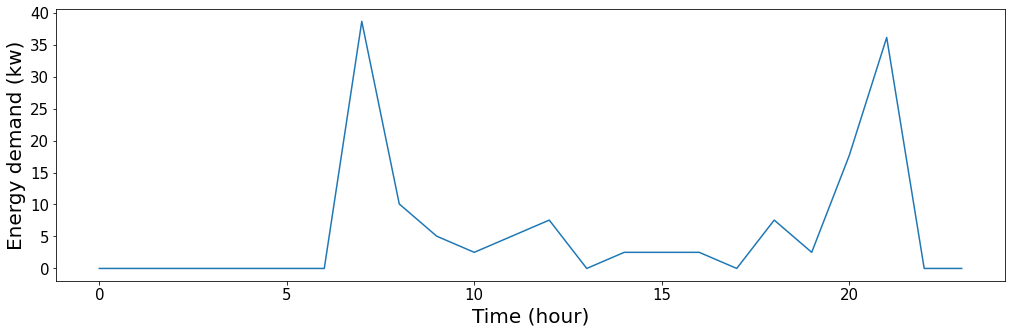
\includegraphics[width=1\columnwidth]{pictures/tap water profile of 24 apartments.png}
\caption[Short title]{Hot tap water use of entire apartment.}
\label{fig:ff11}\end{figure}

The heat demand for the building:

\begin{equation}
Q_{building} = Q_{hotwater} + Q_{heating}
\end{equation}

\begin{figure}[H]
\centering
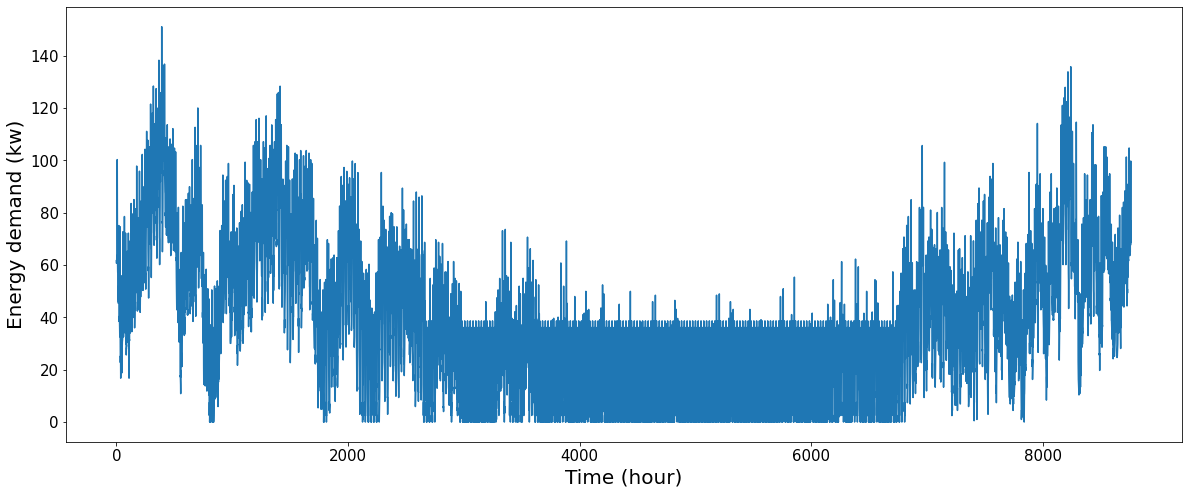
\includegraphics[width=1\columnwidth]{pictures/Q_building profile.png}
\caption[Short title]{Energy demand for an Apartment.}
\label{fig:ff12}\end{figure}

\subsection{BENG and load profile correction}

Total energy consumption for D.H.W with profile M [4] (Appendix A) is 5,845 kwh per day. The annual consumption is therefore approximately 2134 kwh. The value is much higher than the indicated value ( approximately 1600 kwh) for 77m2 apartments from NTA8800 [7], figure 13.

\begin{figure}[H]
\centering
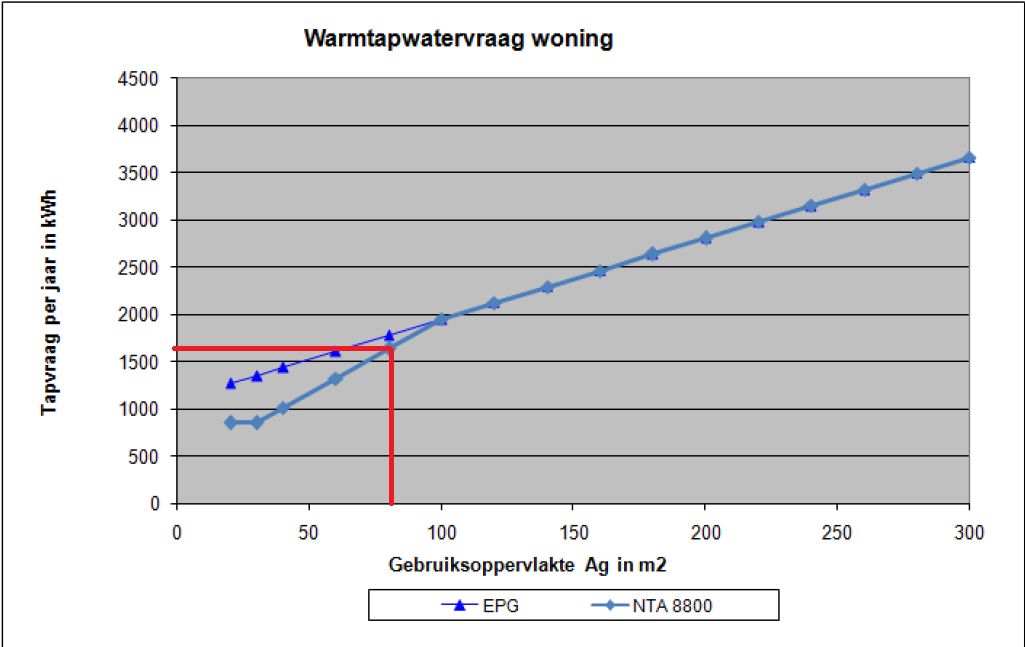
\includegraphics[width=1\columnwidth]{pictures/NTA_8800_DHW.png}
\caption[Short title]{Hot tap water use per year (kwh/$m^2$) [7].}
\label{fig:ff13}\end{figure}

According to NEN 12831-3 [10], Method for calculation of the design heat load - Part 3:  Domestic hot water systems heat load and characterisation of needs. The value of volume of hot water per day ($V_{W;P;day}$) can be calculated based on the number of equivalent persons (adults) $n_{P,eq}$.
\vspace{2mm}
\\
\textbf{Apartment dewellings}.\\
The area is used to calculate $n_{P,eq}$,max as follow: 
\begin{equation}
    n_{P,eq,max}= 1.75 - \begin{cases}
			1, & \text{if $A_{h} < 10 m^2$}\\
            0.01875\cdot(50 - A_h), & \text{if $10 m^2 <A_{h} < 50 m^2$}\\
            0.035\cdot A_h, & \text{if $A_{h} > 50 m^2$}
		 \end{cases}
\end{equation}\\
The total number of equivalent persons is defined by formula:


\begin{equation}
    n_{P,eq}= 1.75 + \begin{cases}
			0.3\cdot n_{P,eq,max}, & \text{if $n_{P,eq,max} < 1.75$}\\
            0.3\cdot(n_{P,eq,max}- 1.75), & \text{if $n_{P,eq,max} \geq 1.75$}
		 \end{cases}
\end{equation}\\
For the residential case and at the level of one dwelling, requirements can be expressed by formula:


\begin{equation}
   V_{W,P,day} = min\Big(x;\Big(y\cdot \frac{A_h}{n_{P,eq}}\Big)\Big)
\end{equation}\\
Where:\\ 
$A_{h}$: habitable area.\\
$n_{P},e_{q}$ number of equivalent persons used for calculating the D.H.W requirements.\\
$n_{P},e_{q,max}$ maximum number of equivalent persons corresponding to the part of the group supplied by the same D.H.W transmitter (individual or attached house and collective housing).\\
The default values for x, and y are:
x = 40,71
y = 3,26 [10]

Applied equations (6) and 7 for the 77m2 apartment dwelling.$n_{P},e_{q}$ = 1.4665.

Compare the assumption of define cases with 2.8 people in 77 $m^2$ there are more likely that the EU-M capacity profile was define for more than 1.4 people,

%________________________________________________________
\section{Associated operating conditions compressor}



%________________________________________________________

\section{ Package of requirements and compressor test plan}

%________________________________________________________


\section{Overview of components with substantiation}






\medskip

%Bibliographic references
\begin{thebibliography}{9}

%______________________

\bibitem{1} 
\texttt{https://www.energievastgoed.nl/benchmarktool/}

%______________________

\bibitem{2} 
\texttt{https://www.energievastgoed.nl/2017/02/14/benchmark-energieverbruik-gebouwen/}


%______________________

\bibitem{3} 
\texttt{Ontwikkeling energiekentallen utiliteitsgebouwen,Een analyse van 24 gebouwtypen in de dienstensector en 12 industriële sectoren, J.M. Sipma, M.D.A. Rietkerk, Januari 2016, ECN-E--15-068}

%______________________


\bibitem{4} 
\texttt{VERORDENING (EU) Nr. 814/2013 VAN DE COMMISSIE
van 2 augustus 2013
tot uitvoering van Richtlijn 2009/125/EG van het Europees Parlement en de Raad wat eisen inzake
ecologisch ontwerp voor waterverwarmingstoestellen en warmwatertanks betreft}

%______________________


\bibitem{5} 
\texttt{Voorbeeldwoningen 2011 Bestaande bouw}

%______________________

\bibitem{6} 
\texttt{KENNISBANK.ISSO.NL, ISSO-publicatie 55,  01-06-2013, ISBN: 978-90-5044-250-3}


%______________________
\bibitem{7} 
\texttt{Nederlandse technische afspraak, NTA 8800, Energieprestatie van gebouwen - Bepalingsmethode, Vervangt NTA 8800:2019-06, ICS 91.120.10; 91.140.30, juli 2020}


%______________________

\bibitem{8} 
\texttt{ECOdesign, meer dan een
label, 20 TVVL Magazine | 03 | 2014 REGELGEVING}

%______________________


\bibitem{9} 
\texttt{\href{https://eur-lex.europa.eu/legal-content/NL/TXT/HTML/?uri=CELEX:32013R0812&from=EN}{https://eur-lex.europa.eu}}

%______________________


\bibitem{9} 
\texttt{NEN-EN 12831-3, Energy performance of buildings - Method for
calculation of the design heat load - Part 3:
Domestic hot water systems heat load and
characterisation of needs, Module M8-2, M8-3}

\end{thebibliography}

%%____________ Appendix_______________________


\begin{appendices}
  \section{Hot tap water profile}

Since september 26, 2015, the Ecodesign [8] and energy labeling guidelines,also apply to appliances for the production of domestic hot water. Devices that do not comply with these guidelines may no longer be sold. In figure 5 the tap water profile label has been highlighted with red square.\\
 

 \begin{figure}[H]
\centering
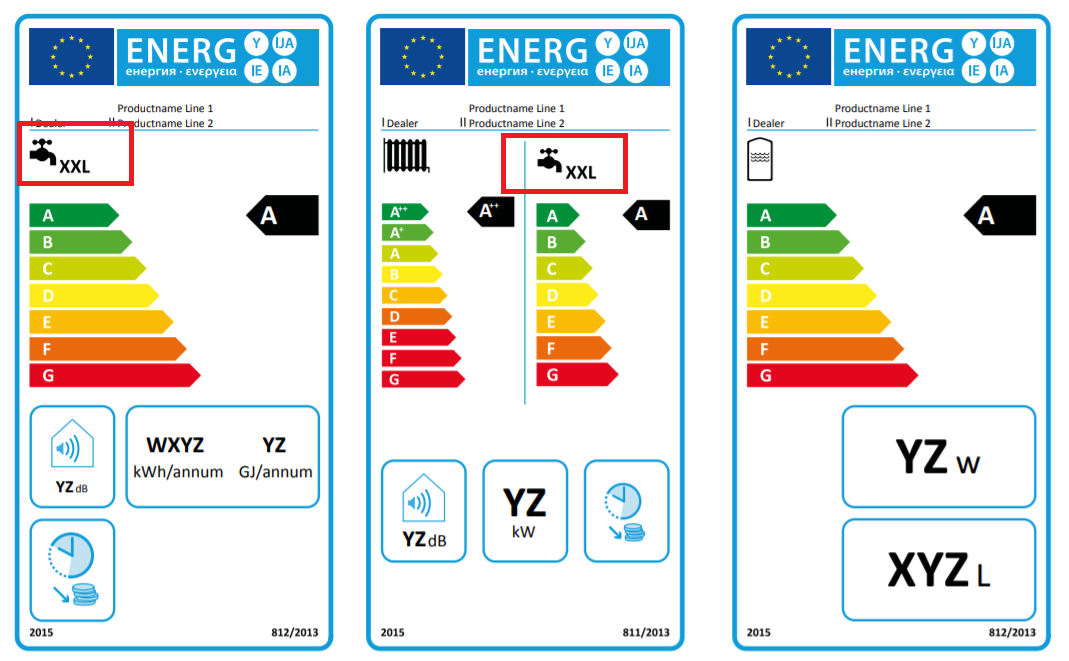
\includegraphics[width=1\columnwidth]{pictures/energy label.png}
\caption[Short title]{Energy label[8]}
\label{fig:ff7}\end{figure}
The hot water classes are defined in the EU regulation with different category label. For example hot water class with label "XL" must be able to supply 18 kWh of hot water per day (1 kWh corresponds to 64.8 MJ heat). This EU regulation also stipulates what conditions hot tap water class must be met.
Figure 8 show that tap water profile for showering can only be selected from label S to XXL.

 \begin{figure}[ht]
\centering
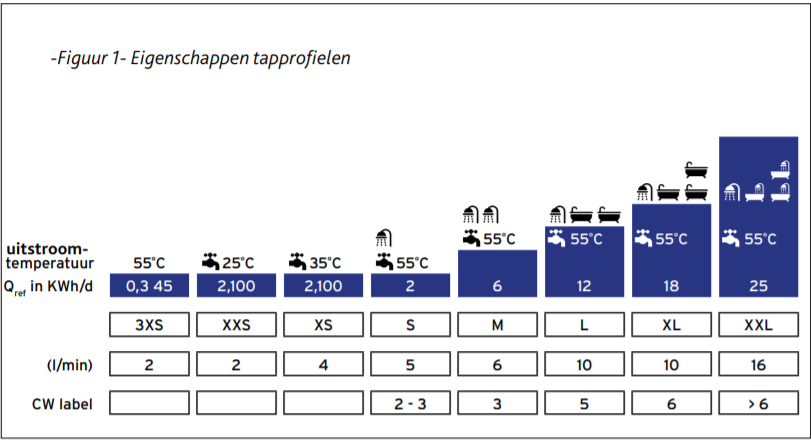
\includegraphics[width=1\columnwidth]{pictures/tap profile.png}
\caption[Short title]{hot water profile labels[8].}
\label{fig:ff8}\end{figure}

  
\begin{figure}[H]
\centering
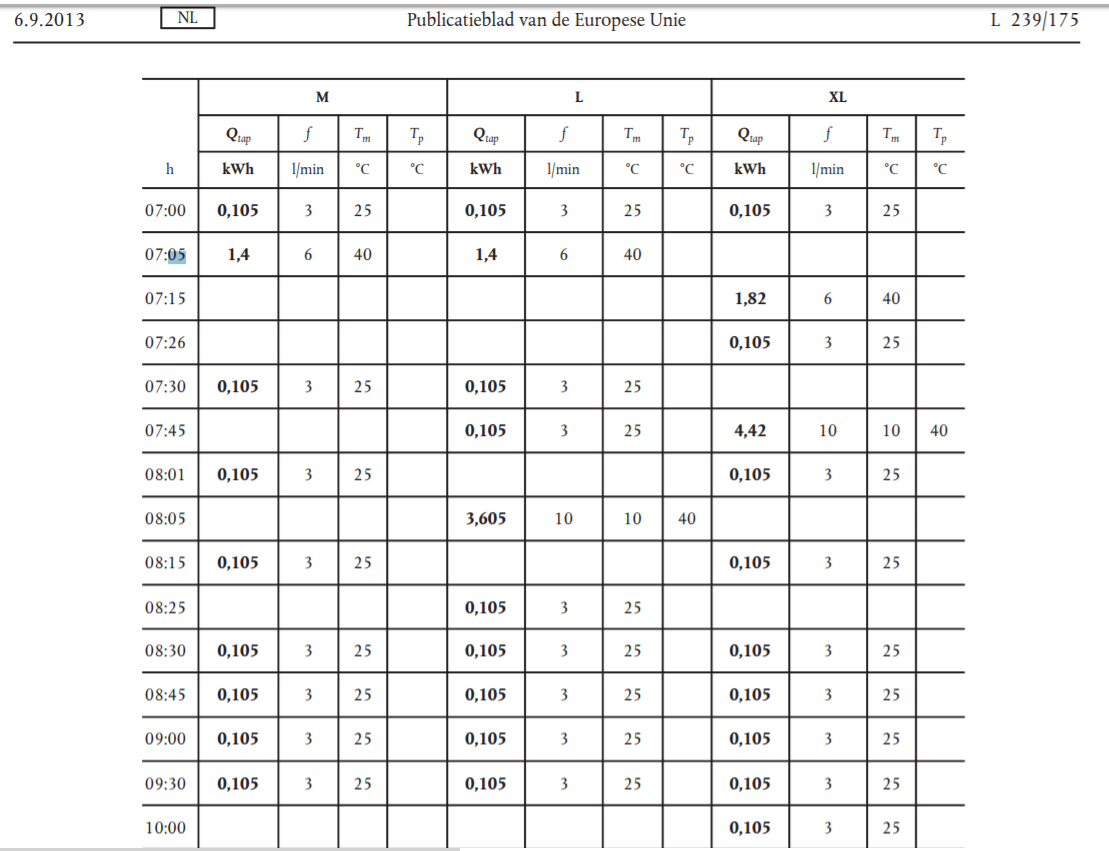
\includegraphics[width=1\columnwidth]{pictures/Profile_M1.png}
\caption[Short title]{Capaciteitsprofielen van waterverwarmingstoestellen.}
\label{fig:ff15}\end{figure}
  
\begin{figure}[H]
\centering
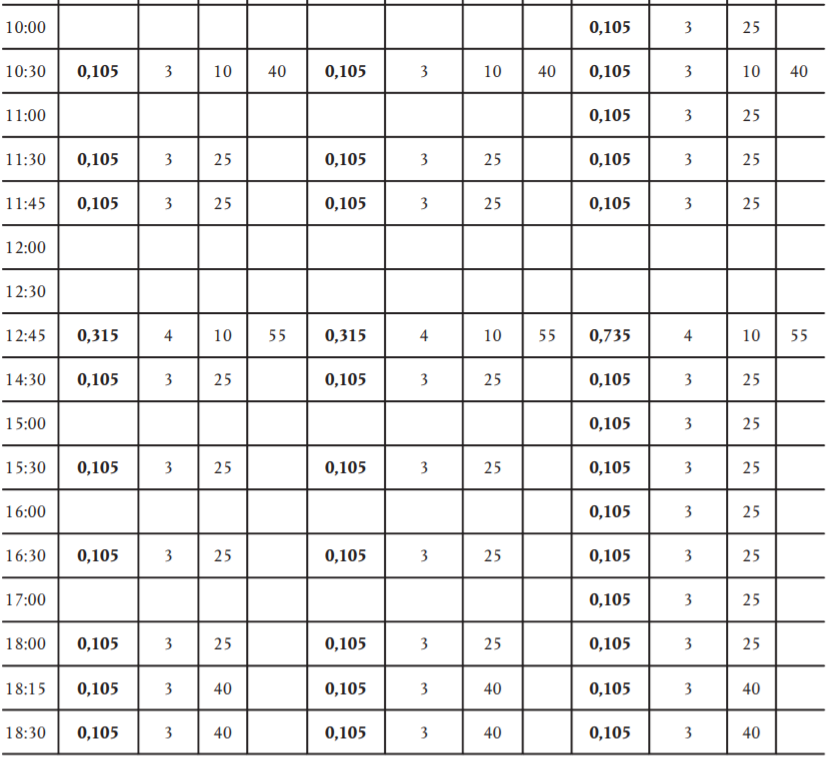
\includegraphics[width=1\columnwidth]{pictures/Profile_M2.png}
\caption[Short title]{Capaciteitsprofielen van waterverwarmingstoestellen.}
\label{fig:ff16}\end{figure}

\begin{figure}[H]
\centering
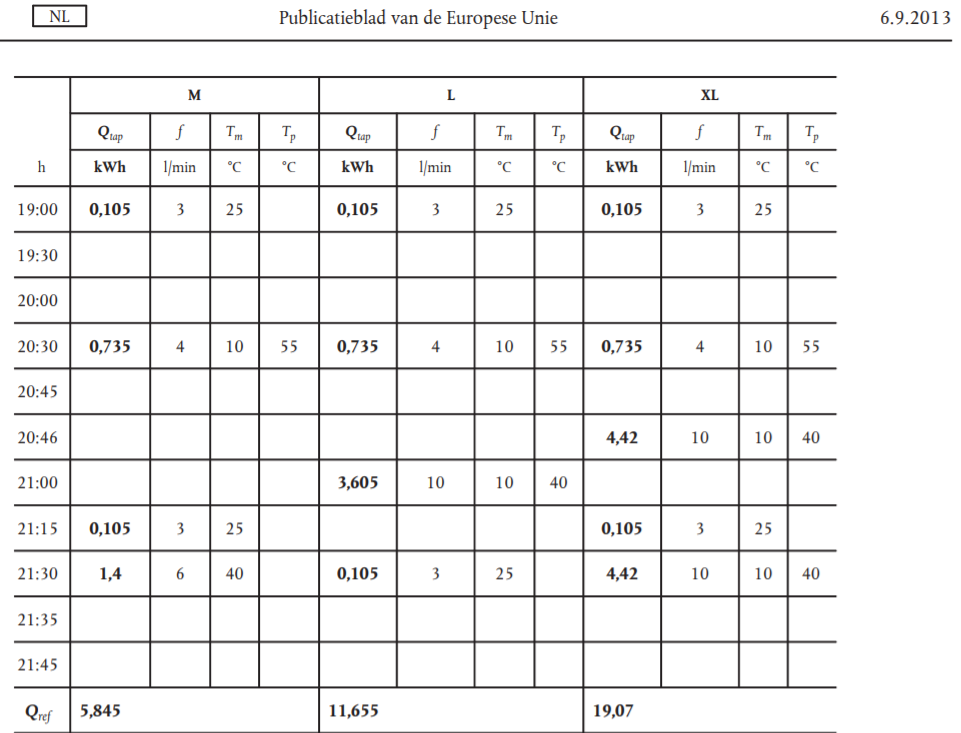
\includegraphics[width=1\columnwidth]{pictures/Profile_M3.png}
\caption[Short title]{Capaciteitsprofielen van waterverwarmingstoestellen.}
\label{fig:ff17}\end{figure}

%____________________________________________________

\section{Calculation methods}

Hot tap water profile for apartments building with 24 residential houses.
From equation (4):

\[V_{WW;60} = 243 + 67.9\sqrt{n} + 12.8n\]

Applied for n = 4 and n = 24

\[ratio =\frac{V_{WW;60;24}}{V_{WW;60;1}}\]
\[f_{new} =f.ratio\]
$f_{new}$: new water flow rate.\\
Look at figure 9 for an example.The amount of water use (litter)

\[m = \frac{3600.Q_{tap}}{c.\Delta T}\]

The time period that water has been used (hour)
\[water_{usetime} = \frac{m.24}{f_{new}.60}\]

Energy use per hour for 24 apartments:

\[Q_{tap/perhour} = 24.Q_{tap}.water_{usetime}\]

\[Q_{building} = Q_{hotwater} + Q_{heating}\]

with $Q_{tap/perhour} = Q_{hotwater}$


  
\end{appendices}


\end{document}

% The D.H.W does not match between profile and year annual consumption.
